%LaTeX source for the ACL 2011 Demo submission for the Topical Guide project
% -abs: Though topic models reduce dimensionality --> Although topic models can be employed for dimensionality reduction
% 
% -abs: their output is just as large as the training corpus. --> their token-level output is as voluminous as the original data set.
% 
% -abs: make these texts usable --> make information in these texts discoverable and thereby usable
% 
% -abstract, sec1, and/or sec9: I think we need to say something about how when you first encounter a large corpus, because you cannot read it, you may not even know what the predominant themes are.  Topic models expose the dominant themes, and the Topical Guide makes it possible to explore what the topic analysis has revealed.
% 
% -sec1: However, when inferred by means of sampling, these models output a topic assignment per token, resulting in an output that is a corpus unto itself. -- delete "when inferred by means of sampling"; the ensuing statement is true whether or not MCMC is the chosen inference method.
% 
% -sec1: very vastness of topic model output --> very vastness of token-level topic model output
% 
% -sec1: this sort of presentation unconvincing. --> this sort of presentation unconvincing and of limited utility.
% 
% -sec1: Simultaneously, massive digitization efforts by libraries -- precede with paragraph break
% 
% -sec1: This constitutes 223 documents totalling XXXXXXX tokens. -- add: "Although this is a small corpus, the Topical Guide has been applied to data sets containing hundreds of thousands of documents." (this is a reference to the student ratings corpus)
% 
% -sec3: or as axes in charts as discussed in section 5. --> or as independent variables for plots, as discussed in section 5.
% 
% -sec4: these include things such as the entropy --> these include metrics such as the entropy
% 
% -sec6: what sets our topic maps apart from the work of Newman et al.?  Let's try to say at least one thing that does.
% 
% -sec6: In the final rendering of the image, edges are omitted to reduce visual complexity. -- perhaps the first order edges from the center topic could be reintroduced, with second order edges still omitted; when I look at the graphs without edges, it seems that something is missing.
% 
% -sec9: It demonstrates the ability of topic modeling to provide highly usable online access to otherwiseobscure document collections. --> The Topical Guide demonstrates the ability of topic modeling to improve discoverability in and provide usable online access to otherwise obscure or overwhelmingly document collections.
% 
% More feedback: figure 5 could be improved to reflect both the procedural steps involved and the products of those steps.  I also think that figure 5 deserves a little more narration.

%In case we change the name of the build script, we define a macro for it:
\newcommand{\buildscript}{backend.py}
\newcommand{\tool}{Topical Guide}
\newcommand{\projecturl}{http://nlp.cs.byu.edu/topicalguide}

\documentclass[11pt]{article}
\usepackage{acl-hlt2011}
\usepackage{times}
\usepackage{latexsym}
\usepackage{amsmath}
\usepackage{multirow}
\usepackage{url}
\usepackage{graphicx}
\usepackage{listings}
\DeclareMathOperator*{\argmax}{arg\,max}
\setlength\titlebox{6.5cm}    % Expanding the titlebox

\title{Increased Comprehension of Topic Models and Corpora\\ Using the \tool}
\author{Josh Hansen, Matthew J. Gardner, Jeff Lund, Dan Walker, Eric Ringger, \and Kevin Seppi\\
Department of Computer Science\\
Brigham Young University\\
\tt \{mjg82,jlutes,joshhansen\}@byu.edu, \{jefflund,danwalkeriv\}@gmail.com\\
\tt \{ringger,kseppi\}@cs.byu.edu}

\begin{document}
\maketitle

\begin{abstract}
Though topic models reduce dimensionality, their output is just as large as the
training corpus. Thus, humans' ability to manually assess model quality is
limited. As the quantity of digitized documents worldwide continues to expand,
institutions correspondingly find an increased need for tools such as topic
models to make these texts usable. In response to these twin needs, we present
the \tool, an open-source web application for interactive,
topic-centric exploration and visualization of topic model output. We explain
why such a tool is warranted, what it is capable of, and how to use it to
explore the corpus or topic model of your choice.
\end{abstract}

\section{Introduction}
Since its introduction, LDA-based topic modeling \cite{blei_latent_2003} has
become standard fare for those wishing to automatically distill large text
collections into something more immediately useful to humans and computers
alike. The usefulness of this sort of dimensionality reduction is widely
acknowledged, and topic models continue to be extended into exciting new
territory.
\cite{wang_continuous_2008,mimno_polylingual_2009,boyd-graber_holistic_2010,brody_unsupervised_2010,he_detecting_2009,yao_efficient_2009}
However, when inferred by means of sampling, these models output a topic
assignment per token, resulting in an output that is a corpus unto itself.
Though the range of possible values is substantially reduced, output size
remains on the same order as input size. Notwithstanding, papers introducing new
topic models often lean heavily on the hope that displaying a few hand-picked
topics will convince others of the model's effectiveness. But the very vastness
of topic model output renders this sort of presentation unconvincing.
Unfortunately, tools for deep understanding of topic model output have thus far
been lacking.
\begin{figure*}[t]
 \centering
 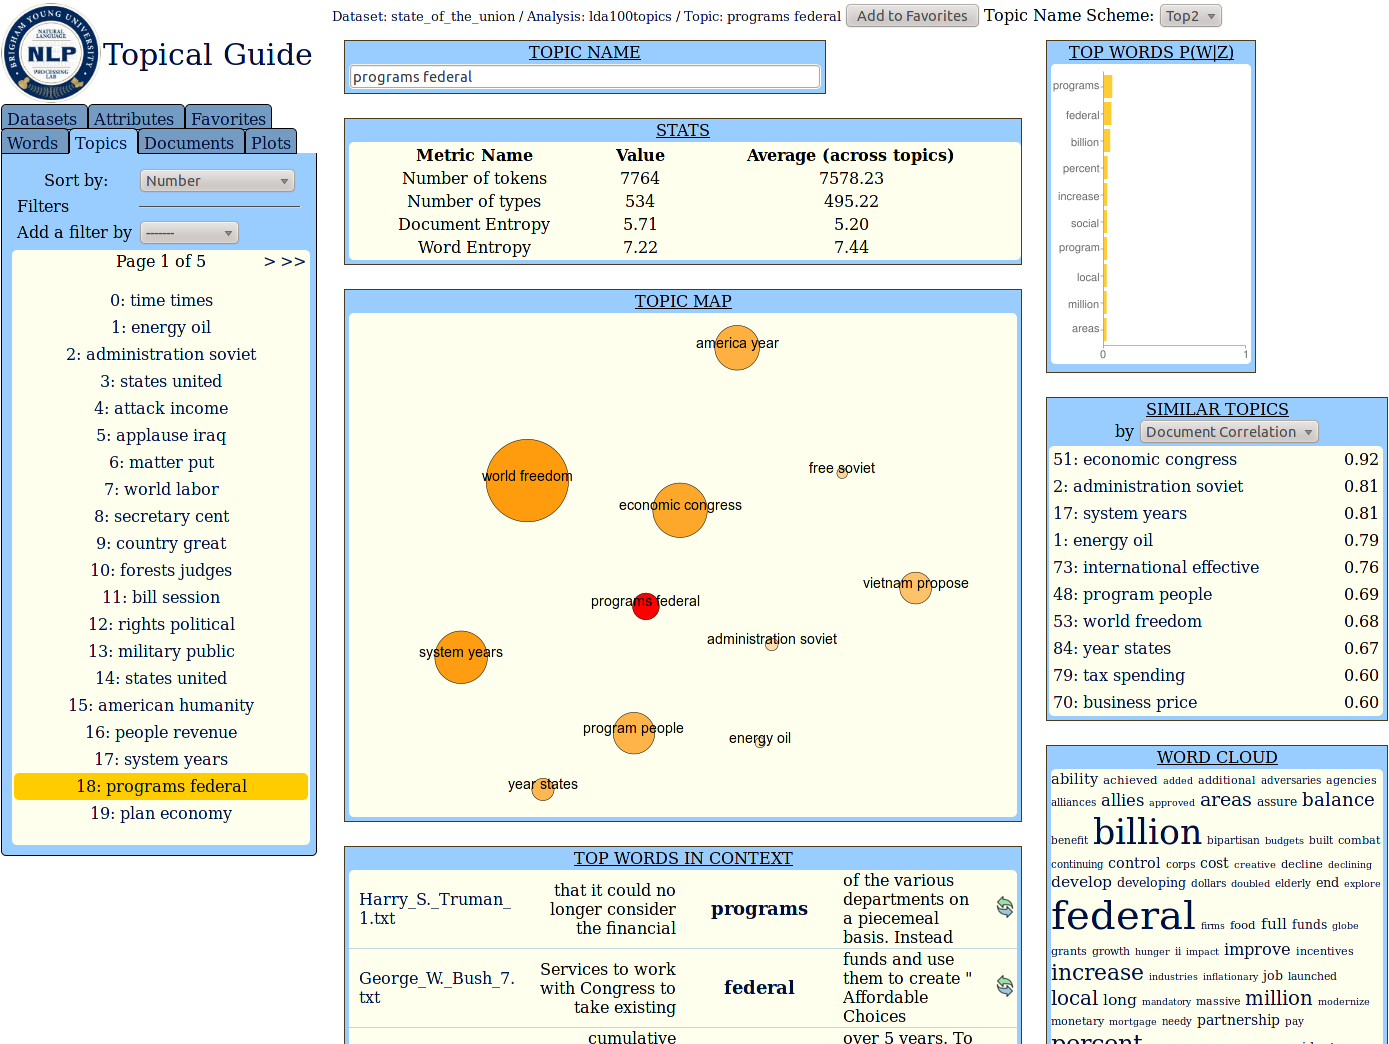
\includegraphics[width=400px,keepaspectratio=true]{./topic_page_take4.png}
 % topic_page_huge_cropped.png: 1394x1027 pixel, 96dpi, 36.88x27.17 cm, bb=0 0 1045 770
 \caption{The topic view}
 \label{fig:topic_page}
\end{figure*}
Simultaneously, massive digitization efforts by libraries and other institutions
are generating gargantuan quantities of electronic text, increasing demand for tools such as
topic models. Because of their ability to characterize the contents of
corpora, topic models seem to hold great promise for archival
institutions wishing to make their newly-digitized collections accessible to
researchers and the public. However, readily available tools for exploration of 
document collections in terms of topic models have been either unsatisfactory
or nonexistent.

In response, we present the \tool, an open-source\footnote{Licensed under the terms of the Affero
General Public License, version 3.} web application for interactive,
topic-aware exploration and visualization of both document collections and the
topic models inferred on them.\footnote{Further information on the project, including
source code access and a live demonstration server, can be found
at \texttt{\projecturl}.} The \tool{} is an aid both to those who wish to
browse through a corpus and for those who wish to analyze the topic model itself.
We believe that this interactive, topic-aware approach to corpus and model exploration
exposes meaningful patterns to human comprehension in a way that static visualizations cannot.

In this paper, we will discuss: browsing of topic model output using the \tool{} user interface, as in \cite{gardner_browser_2010};
document metadata; document and topic metrics; a topic-space visualization;
topic name schemes; and the data import
system. Throughout this paper, examples are taken from a
corpus of State of the Union messages delivered by United States presidents
from 1790 to 2010. This constitutes 223 documents totalling XXXXXXX tokens. %TODO Count tokens

\begin{figure*}[t]
 \centering
 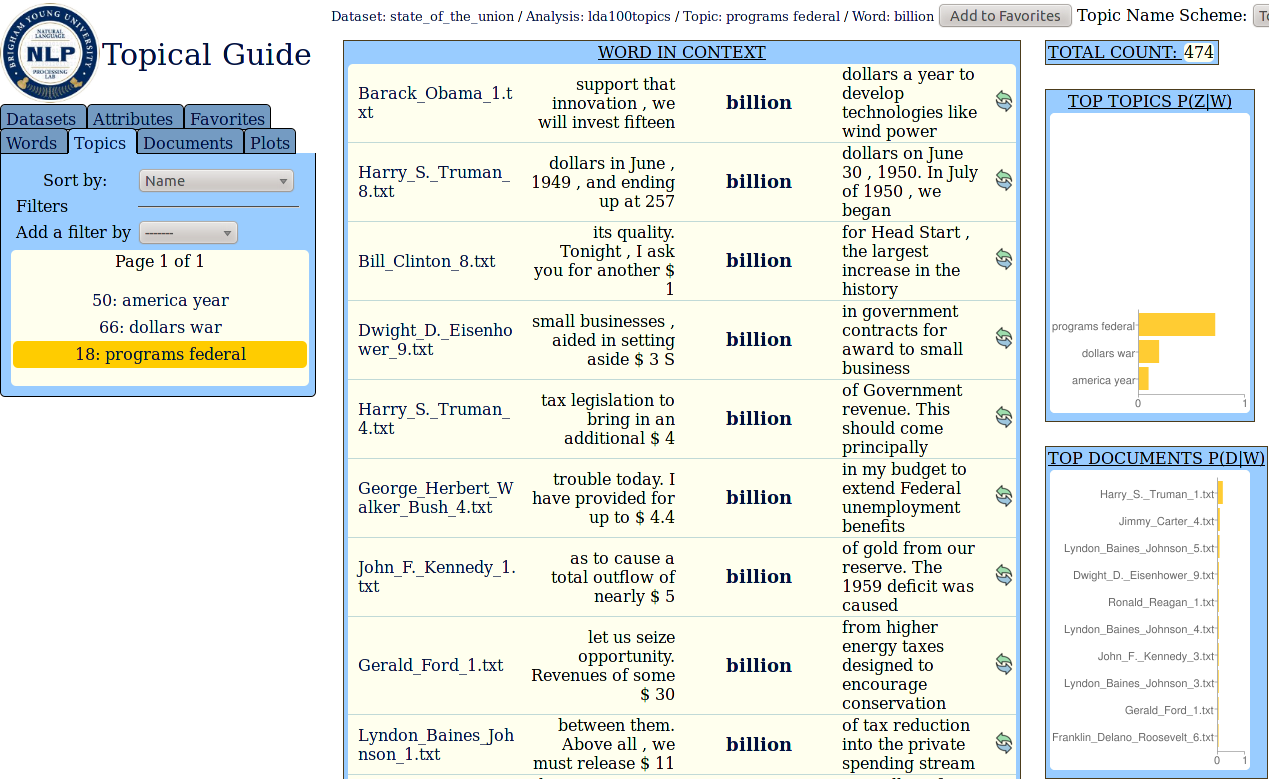
\includegraphics[width=400px,keepaspectratio=true]{./topic_word_view2.png}
 % topic_document_view.png: 1359x858 pixel, 96dpi, 35.95x22.70 cm, bb=0 0 1019 643
 \caption{A view of the word ``billion'' as it occurs in the ``programs federal'' topic.}
 \label{fig:topic_word}
\end{figure*}
\section{Browsing}
All entities explicitly modeled by a basic topic model---topics, documents,
and words---are first-class citizens in the \tool, meaning that the user
interface provides specific views for each of these entity types. The topic view
is central to the user experience. A view of the ``programs federal'' topic is
rendered in Figure \ref{fig:topic_page}. On the left is a navigation sidebar listing other topics,
with tabs providing links to other views such as Attributes, Documents, and Plots.
The remainder of the page shows statistics about the topic
(\texttt{STATS}); chart, word-cloud, and key-word-in-context representations of top
words (\texttt{TOP WORDS P(W|Z)} / \texttt{WORD CLOUD} / \texttt{TOP WORDS IN CONTEXT}); and
both textual and graphical representations of similar topics (\texttt{SIMILAR
TOPICS} / \texttt{TOPIC MAP}).

The word view is shown in Figure \ref{fig:topic_word}. It presents the user with
a list of contexts in which the word appears, along with the total number of
occurrences, and lists of topics and documents in which the word occurs most
often. 

The document view can be seen in Figure \ref{fig:topic_doc}, showing the content
of the document along with prominent topics and any document metrics that have been computed. By
means of pairwise document metrics, a list of similar documents is shown as
well.

Intuitive hyperlinks facilitate an interactive experience. Click on the
``economic congress'' node in the topic map and be sent to its topic view
to see how presidents have discussed economic issues. Click on ``billion'' in
the word cloud to see how that word has been used in various addresses (Figure
\ref{fig:topic_word}). Or click on ``Harry\_S.\_Truman\_1.txt'' to see
President Truman's message with words belonging to the ``programs federal''
topic highlighted (Figure \ref{fig:topic_doc}).
%TODO Make words in the doc view link
%TODO Show words in context in the word view

% An important concept used by the \tool{} object model and user interface is the
% notion of \textit{datasets} and \textit{analyses}. A dataset is a set of
% documents --- a corpus. An analysis is associated with one dataset and
% constitutes a set of topics and token-level topic assignments for all of the
% documents in that dataset. The analysis concept is useful in allowing for
% multiple topic models on a single dataset. For example, it could be useful to
% use LDA to infer both a 20-topic model and a 100-topic model on the State of the
% Union Addresses dataset.

\begin{figure*}[t]
 \centering
 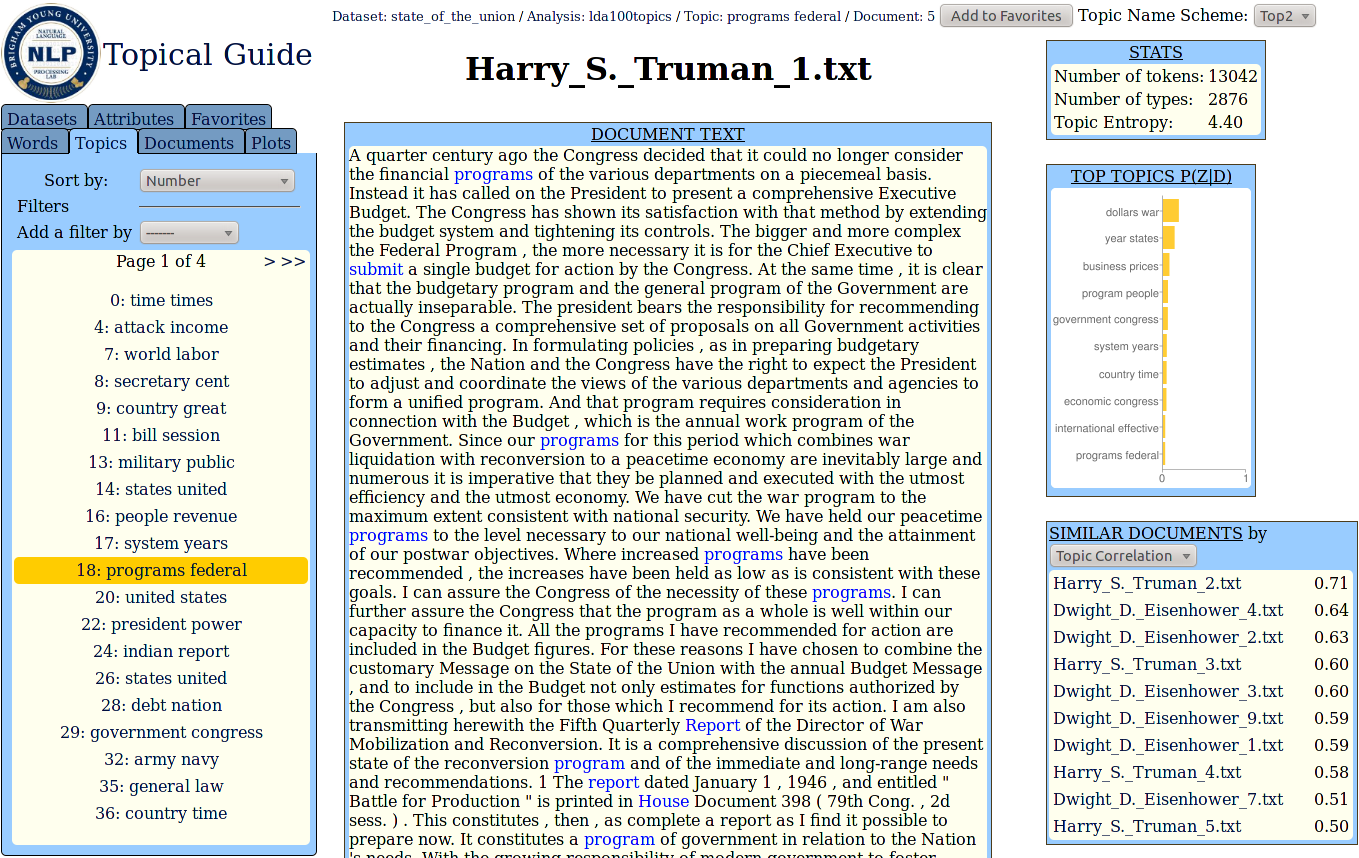
\includegraphics[width=400px,keepaspectratio=true]{./topic_document_view.png}
 % topic_document_view.png: 1359x858 pixel, 96dpi, 35.95x22.70 cm, bb=0 0 1019 643
 \caption{A view of Harry Truman's first State of the Union address, highlighting words belonging to the ``programs federal'' topic.}
 \label{fig:topic_doc}
\end{figure*}

\section{Document Metadata}
Acknowledging that more is known about most documents than just their content,
the \tool{} provides \textit{document attributes}, a mechanism for association
of arbitrary metadata with documents. This accomodates metadata
provided by a dataset curator, often including facts about document
provenance and author identity. Document attributes also allow for metadata
obtained as part of the output of a model. These attributes can be used to
filter the list of documents, or as axes in charts as discussed in section \ref{sec:plots}.

\section{Metrics}
Topic-centric document exploration is enhanced by means of \textit{metrics}.
Metrics are functions that give users additional insight into the nature of
topics or documents. Topic metrics range from
simple metrics, such as the number of word tokens and types labeled with the
topic, to more complicated metrics such as dispersion across documents,
prevailing sentiment, or the semantic coherence of its words \cite{Newman2010Coherence}.

\textit{Pairwise} topic metrics describe relationships between
topics.\footnote{Pairwise metrics do not necessarily constitute
``metrics'' in the formal sense. We leave it to implementers to determine
whether to satisfy the triangle inequality, etc.} These include Pearson correlation on documents and on words.
Pairwise metrics are used to automatically display a list of similar topics and to weight
the edges of the graph used to generate topic maps (discussed further in section
\ref{sec:maps}).

Similar to topic metrics, document metrics can also be computed.
Beyond simple metrics like token count in the document, these include
things such as the entropy of the topic distribution of the document \cite{Misra2008}. As
with topics, we make use of pairwise document metrics such as topic
correlation \cite{Blei2009} to show similar documents.

\begin{figure*}[t]
 \centering
 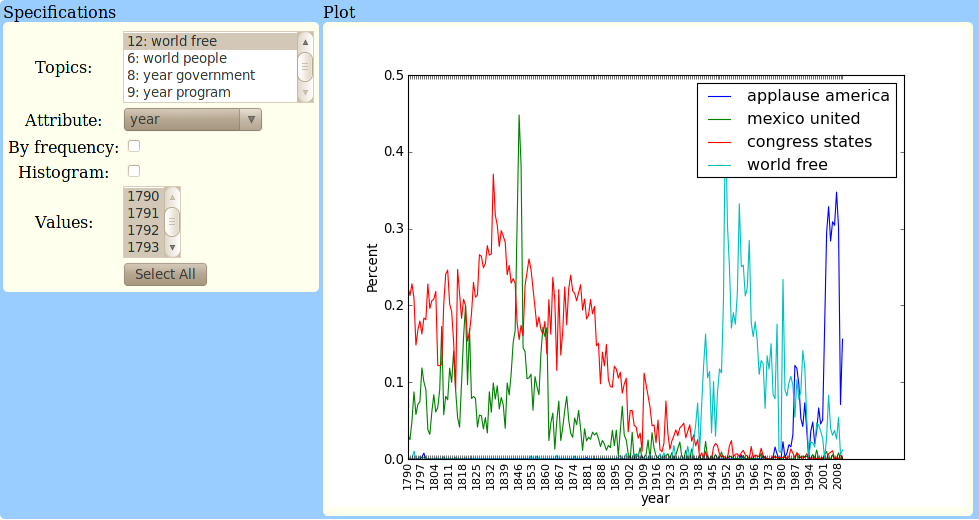
\includegraphics[height=200px,keepaspectratio=true]{./topics_vs_years.png}
 % topics_vs_years.png: 979x520 pixel, 96dpi, 25.90x13.76 cm, bb=0 0 734 390
 \label{fig:chart}
 \caption{Selected topics over time as a percentage of overall tokens.}
\end{figure*}

\section{Plots}\label{sec:plots}
The \tool{} allows users to interactively generate two types of plots. The first
shows topic trends over the values of an attribute---for example, the year
of an address, or the political party of the president delivering it. This kind
of plot has been used in visualizing topic models almost since their
introduction. In our system they can be generated over any attribute for any
topic or combination of topics in the corpus. Figure \ref{fig:chart} shows
trends for four chosen topics across the ``year'' attribute, giving a view
of topic lifecycles across time as in \cite{Griffiths2004,Wang2006}.

The second type of plot is a scatter plot of topic metrics, by which one topic
metric is plotted against another. This is particularly suited to discovery of
relationships between topic metrics. For example, we have found that document
entropy seems to correlate with the logarithm of the number of tokens in the
topic, and that coherence does not seem to correlate with any other topic metric
yet implemented.

\section{Topic Maps}\label{sec:maps}
With topic-to-topic relationships described by means of pairwise topic metrics,
graph-based visualization of the topic space becomes straightforward. We
integrate the topic maps into an overall browsing experience to help users
quickly assess how topics relate to each other. In our current implementation, we
construct a topic graph $G = (N, E)$ for a set of topics $T$ as follows:

$N$ is a set of $|T|$ nodes such that
\[\forall_{t\in T} weight(N_{t}) = \tau_{1}(t)\]
and
\[\forall_{t\in T} color(N_{t}) = \tau_{2}(t)\]
where $\tau_1$ and $\tau_2$ are topic metrics (potentially the same). $E$ is
constructed as a set of $|T|^2$ edges such that
  \[\forall_{(t,u)\in T\times T, t\neq u} weight(E_{t,u}) = \pi(t,u)\]
where $\pi$ is a pairwise topic metric.

Figure \ref{fig:topic_page} shows such a graph as part of a topic view. We use
the Gephi Toolkit\footnote{http://www.gephi.org} to generate the graphs and
render them as images, employing a force-directed layout algorithm to arrange
the nodes so that, generally speaking, nodes joined by edges of higher weight
are closer together, and nodes joined by edges of lower weight are further
apart. (A similar approach focused on visualization of the document space is
described in \cite{Newman2010Maps}.) In the final rendering of the image, edges
are omitted to reduce visual complexity. However, the distances between nodes
are still determined by the interaction of the layout algorithm and the edge
weights.

\section{Topic Name Schemes}
As LDA does not assign names to the topics it generates, automatic generation of
topic names is of interest to researchers wishing to make topic models
human-usable. Research in this area is ongoing \cite{Mei2007,Lau2010}. In order to
facilitate investigations in this area, we equipped the \tool{} with a
fully pluggable topic naming system. Any number of topic name schemes can be
used to produce names for all topics in a model. Within the user interface
users can select a name scheme, which is then reflected throughout the
interface. By default we use a concatenation of the two
words with the highest probability for a given topic, and alternative schemes
can be imagined and easily implemented.%TODO Maybe show TF-ITF?

\begin{figure*}[ht]
 \centering
 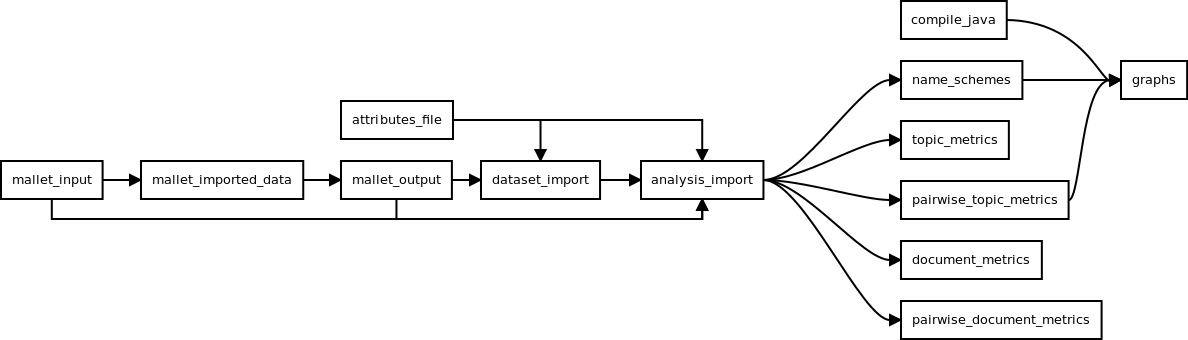
\includegraphics[width=400px,keepaspectratio=true]{./build_flowchart2.png}
 % build_deps.png: 1188x340 pixel, 72dpi, 41.91x11.99 cm, bb=0 0 1188 340
 \caption{Dependencies within the data import pipeline. Arrows indicate that the source is prerequisite for the target.}
 \label{fig:build_flowchart}
\end{figure*}
\section{Data Import Backend}
Automatically turning a raw document collection into an interactive browsing
experience requires extensive preprocessing. Documents must be converted into a
representation accepted by the topic model learner. Topics must then be inferred
and model output indexed for quick retrieval by the web front-end.
Additionally, metrics must be computed, topic names generated, and graphs rendered
before they become accessible via the user interface. Unsurprisingly, the dependencies
in the import process form a directed acyclic graph, represented in Figure~\ref{fig:build_flowchart}.
In order to make workflows simpler and more efficient, we implemented
the import process as a command-line frontend based on the \texttt{doit}
task automation tool.\footnote{http://doit.sourceforge.net/} This allows full
import of a dataset using a single invocation of the import script.

Enabling the \tool{} to browse a new dataset can be as simple as picking a name
and description, converting the documents to plaintext, placing them in a
directory, and providing a JSON file containing any document metadata. By default,
the \tool{} will automatically invoke MALLET's LDA implementation to train a
topic model \cite{McCallum2002}; however, the import system can also make use of
existing topic model output in the MALLET format. The system also allows all
elements of the pipeline to be overridden, allowing for customization and
clean integration with existing code.

\section{Conclusion}
We have presented the \tool, an open-source web application for interactive,
topic-centric exploration and visualization of topic model output.
This software demonstrates the ability of topic modeling to provide
highly usable online access to otherwise-obscure document collections.
The free availability of such a tool also makes it easy to expose
topic model output to third-parties for scrutiny, implicitly challenging
the field to adopt a higher standard of transparency in future research.

\bibliographystyle{acl}
\bibliography{acl2011demo.bib}
\end{document}

